\begin{itemize}[leftmargin=1em]
\item \textbf{Concentration in interest-rate risk.} Treasuries are the least volatile asset and therefore receive the largest
weight (on average \res{avg_w_ief}). A simultaneous fall of bonds and equities, as in 2022, hits risk parity directly; the trend
filter limited the 2022 loss to \res{strat_ret_2022} but cannot prevent sudden shocks. Adding inflation-linked Treasuries
(TIP) as a seventh asset class hardly helped in the 2022 rate shock (\res{imp_tip_2022} vs \res{strat_infl}) and was not adopted.
\item \textbf{Trend reversals.} After a sharp fall and quick rebound the filter sells late and buys back late. In 2020 the
strategy returned \res{strat_ret_2020} while 60/40 earned \res{b6040_ret_2020}. In strong bull markets the client will often
lag: the strategy beat 60/40 in only \res{years_beating_6040} of \res{n_years_cal} calendar years.
\item \textbf{Look-ahead bias.} Every weight uses only prices up to its decision date; the truncation test of Section~4
confirms this.
\item \textbf{Survivorship and hindsight bias.} We hold broad asset classes instead of picked winners, and their ETFs are
among the largest of their kind. Still, the universe is chosen today. Leaving out any one asset class gives Sharpe ratios
between \res{loo_sharpe_min} and \res{loo_sharpe_max} (worst without \res{loo_worst_asset}; without gold \res{loo_sharpe_nogold})
and a maximum drawdown no worse than \res{loo_maxdd_worst}, so no single holding drives the result.
\item \textbf{Data snooping.} The 10-month average and the one-year risk window are fixed in advance from the literature. Across
all \res{heat_n} combinations of 6--12 months and 3, 6 or 12 months of risk data, the Sharpe ratio stays between \res{heat_min}
and \res{heat_max} (Figure~\ref{fig:sensitivity}): a plateau, not a lucky spike. Because trying many variants makes a good backtest easy to find by
chance \citep{bailey2014pbo}, the machine-learning variants of Section~9 were judged by gates fixed before the first run, so
they could not be tuned towards a better backtest; none of them was adopted.
\item \textbf{Statistical confidence.} In a circular block bootstrap \citep{politis1992} of several thousand resampled histories
(12-month blocks) the strategy's maximum drawdown is smaller than that of 60/40 in \res{ext_boot_p_mdd} of draws, while
its Sharpe ratio is higher in only \res{ext_boot_p_sharpe}: the lower drawdown is robust, the risk-adjusted return is the
same. The Sharpe ratio is similar in both halves of the sample (\res{ext_sub1_sharpe_a} and \res{ext_sub2_sharpe_a}).
\item \textbf{Rebalancing day.} Month-end was the most favourable of four tested rebalancing days. Rebalancing 0, 5, 10 or
15 trading days before month-end gives Sharpe ratios between \res{ext_offset_sharpe_min} and \res{ext_offset_sharpe_max}
and drawdowns of up to \res{ext_offset_mdd_worst}, still far smaller than those of 60/40. Four tranches with these rebalancing
days give \res{imp_m_sharpe}, close to their average; this is the more realistic expectation than the month-end result.
\item \textbf{Out-of-sample test.} As a final check we ran the rule on \res{imp_oos_start}--\res{imp_oos_end}, before the ETFs
existed, with long-history index funds as proxies. No free gold series exists for that period, so five of the six asset
classes are covered. The project had never used these data. The rule had a Sharpe ratio of \res{imp_oos_a_sharpe} and a
maximum drawdown of \res{imp_oos_a_maxdd}, against \res{imp_oos_6040_sharpe} and \res{imp_oos_6040_maxdd} for 60/40. Counting all
\res{imp_n_trials} variants tried in the notebook, the deflated Sharpe ratio \citep{bailey2014} still puts the probability that
the true Sharpe ratio is positive at \res{imp_dsr_a}.
\item \textbf{Short sample, model and data risk.} \res{sample_years} years contain only three major crises; the strategy's
results depend on how future crises unfold. Covariances are estimated with error, Yahoo Finance revises adjusted prices
occasionally, and the backtest assumes trading at closing prices without taxes.
\end{itemize}
\begin{figure}[!htb]
\centering
\caption{Net Sharpe ratio for different trend and risk windows; * marks the base case.}\label{fig:sensitivity}
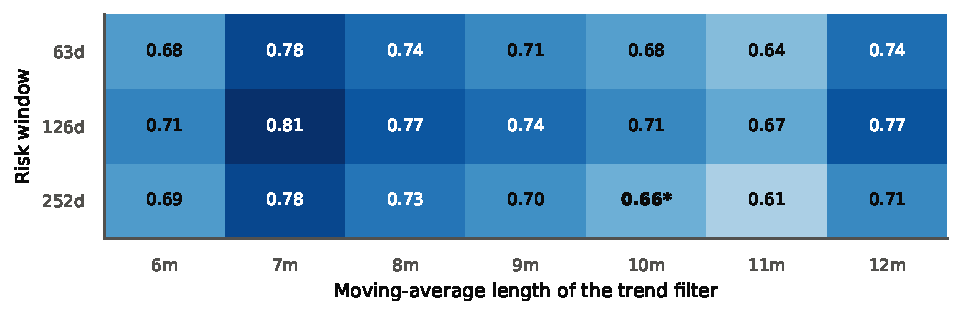
\includegraphics[width=\textwidth]{figures/fig_sensitivity.pdf}\resmark{fig_sensitivity}
\end{figure}
